\documentclass[main.tex]{subfiles}
\begin{document}
\section{Simulation Results}
\label{sec:simulation-results}
Consider the objective trajectory in (\ref{eq:Er-property}) with $l_r = 3\text{m}$ and $\theta_{\max} = 2\pi/5$, giving that $g = 9.81\text{m/s}^2$. The condition in $k_P$ is $k_P > g^2|\cos{\theta_{\max}}| = 29.74$. Choosing 
\begin{equation} \label{eq:control-parameters}
\begin{aligned}
    k_D = 12, && k_P = 30, && k_V = 12
\end{aligned}
\end{equation}
yields $l_{de} = 1.42$ $m$.
\subsection{Total Energy Shaping}
For an initial state $\big(\theta(0),l(0),\dot{\theta}(0),\dot{l}(0)\big) = (-\pi/6,2,0,0)$, 
the numerical simulation results of the VLP under the controller \eqref{eq:tot-mech-energy-controller} using the defined control parameters are shown in Figs. \ref{fig:total_1} and \ref{fig:total_2}. It is observed that $V_c$ and $E_T-E_r$ converge to zero, while $V_c$ is non-increasing. Moreover, the denominator of the controller \eqref{eq:tot-mech-energy-controller}, $E_T-E_r+k_D$ is positive for all $t\geq 0$ as shown in Fig. \ref{fig:total_1}. However for an initial state $\big(\theta(0),l(0),\dot{\theta}(0),\dot{l}(0)\big)$ $= (-\pi/6,2,0,4)$ the denominator $E_T-E_r+k_D$ is positive at $t=0$ and becomes $0$ about $t = 0.16$ $s$, which shows that the controller \eqref{eq:tot-mech-energy-controller} encountered a singular point; as observed in Fig.(\ref{fig:singular_controller}a. This defines the difficulty discussed in choosing the control parameters to avoid singular points in this controller for all initial states.
\begin{figure}[H]
    \centering
    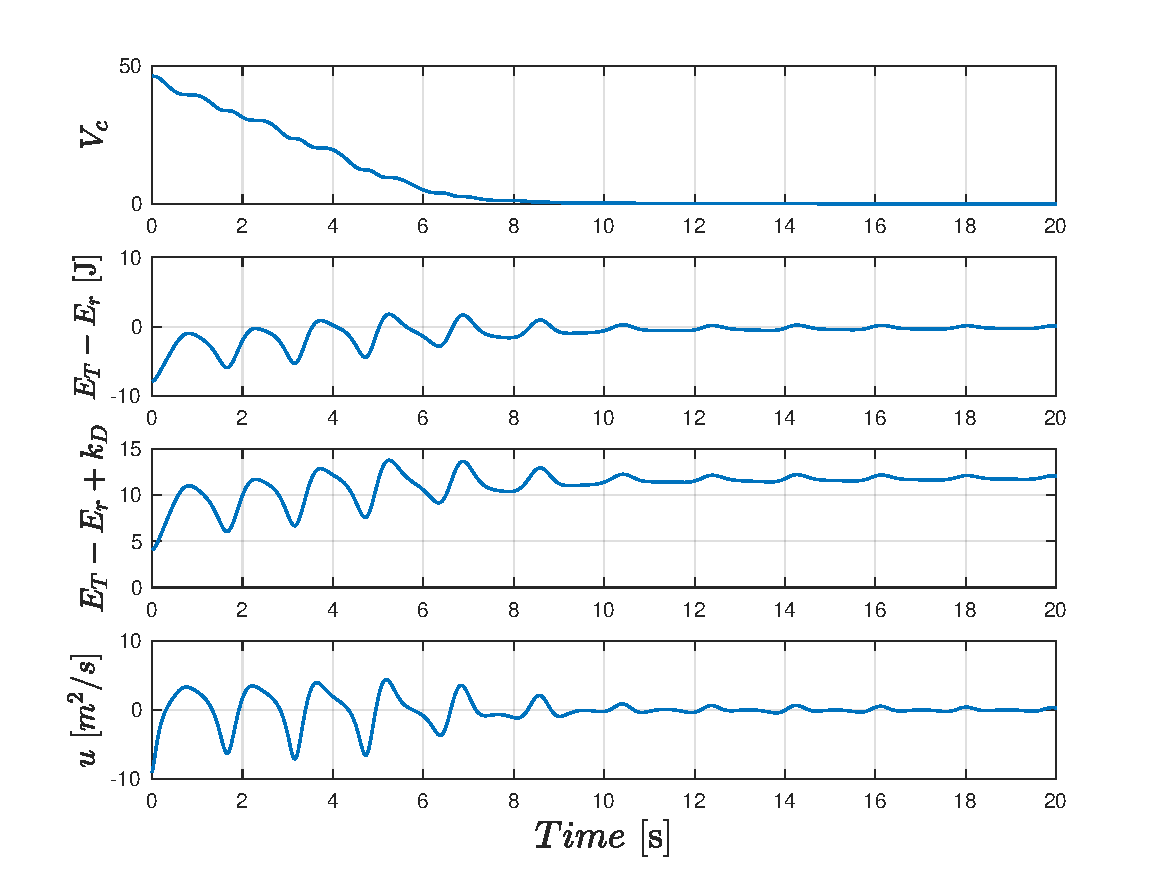
\includegraphics[scale = 0.6]{figures/Total_Energy_Shaping/total_1b.pdf}
    \caption{Time responses of $V_c$, $E_T-E_r$, $E_T-E_r+k_D$
    and $u$ with initial state $\big(\theta(0),l(0),\dot{\theta}(0),\dot{l}(0)\big) = (-\pi/6,2,0,0)$.}
    \label{fig:total_1}
\end{figure}
\begin{figure}[H]
    \centering
    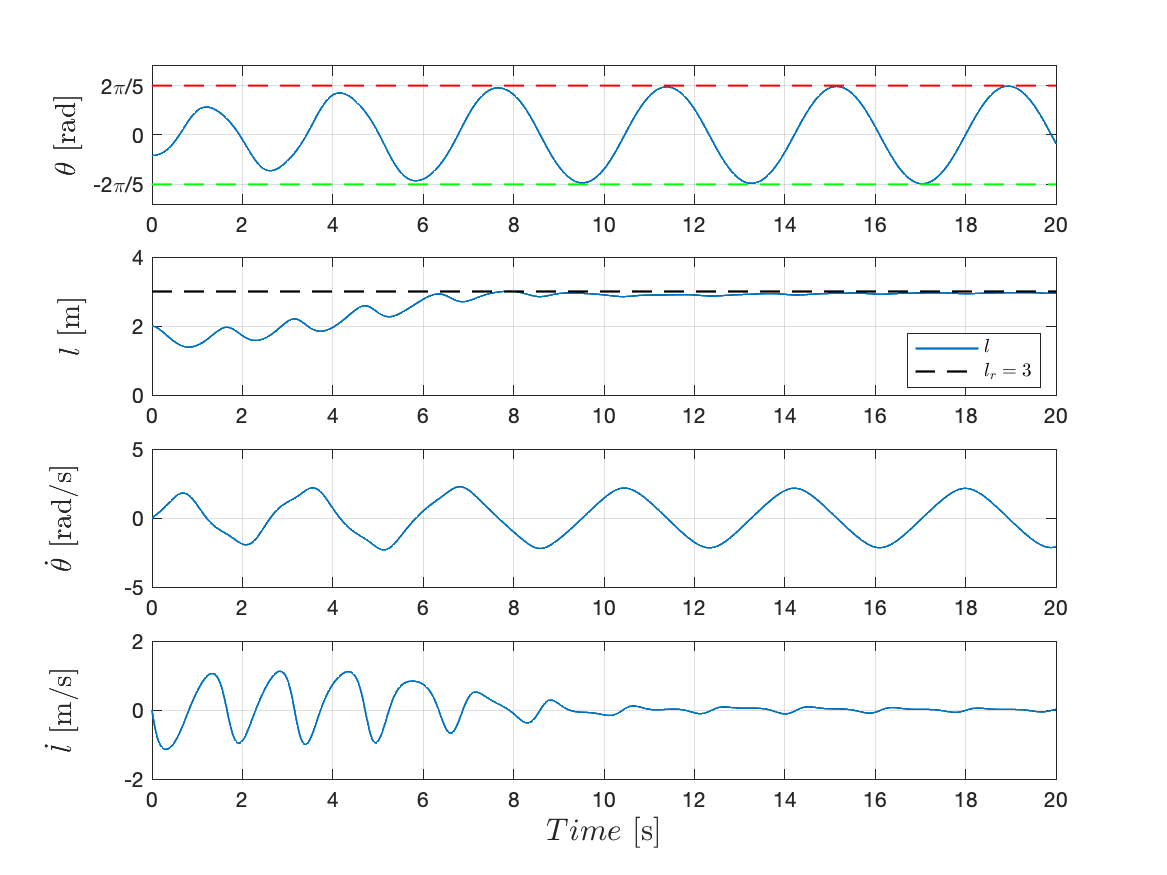
\includegraphics[scale = 0.6]{figures/Total_Energy_Shaping/total_2b.pdf}
    \caption{Time responses of $\big(\theta,l,\dot{\theta},\dot{l}\big)$ with initial state $\big(\theta(0),l(0),\dot{\theta}(0),\dot{l}(0)\big)$ $= (-\pi/6,2,0,0)$.}
    \label{fig:total_2}
\end{figure}
\begin{figure}[H] 
\begin{subfigure}{.5\textwidth}
  \centering
  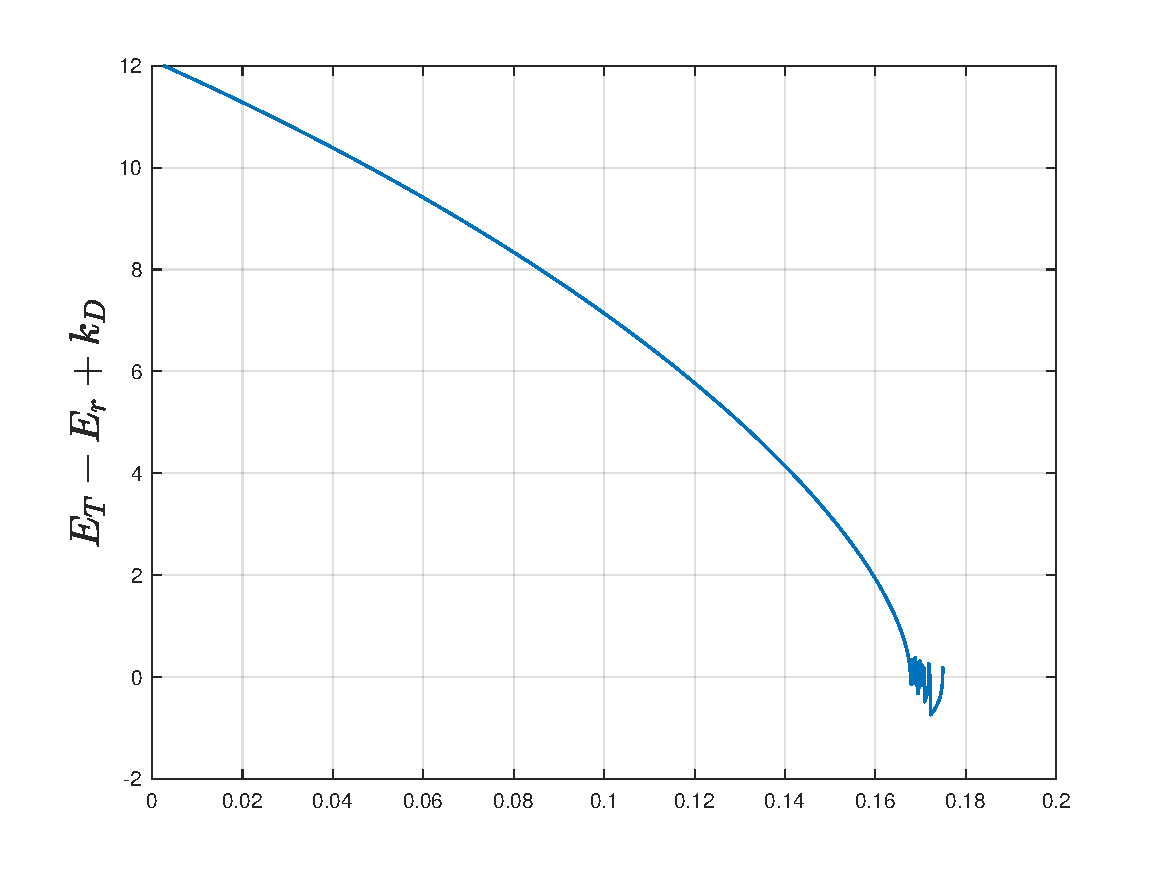
\includegraphics[width=1\linewidth]{figures/Total_Energy_Shaping/total_2.pdf}
\caption{Time responses of $E_T-E_r+k_D$.}
\end{subfigure}
\begin{subfigure}{.5\textwidth}
  \centering
  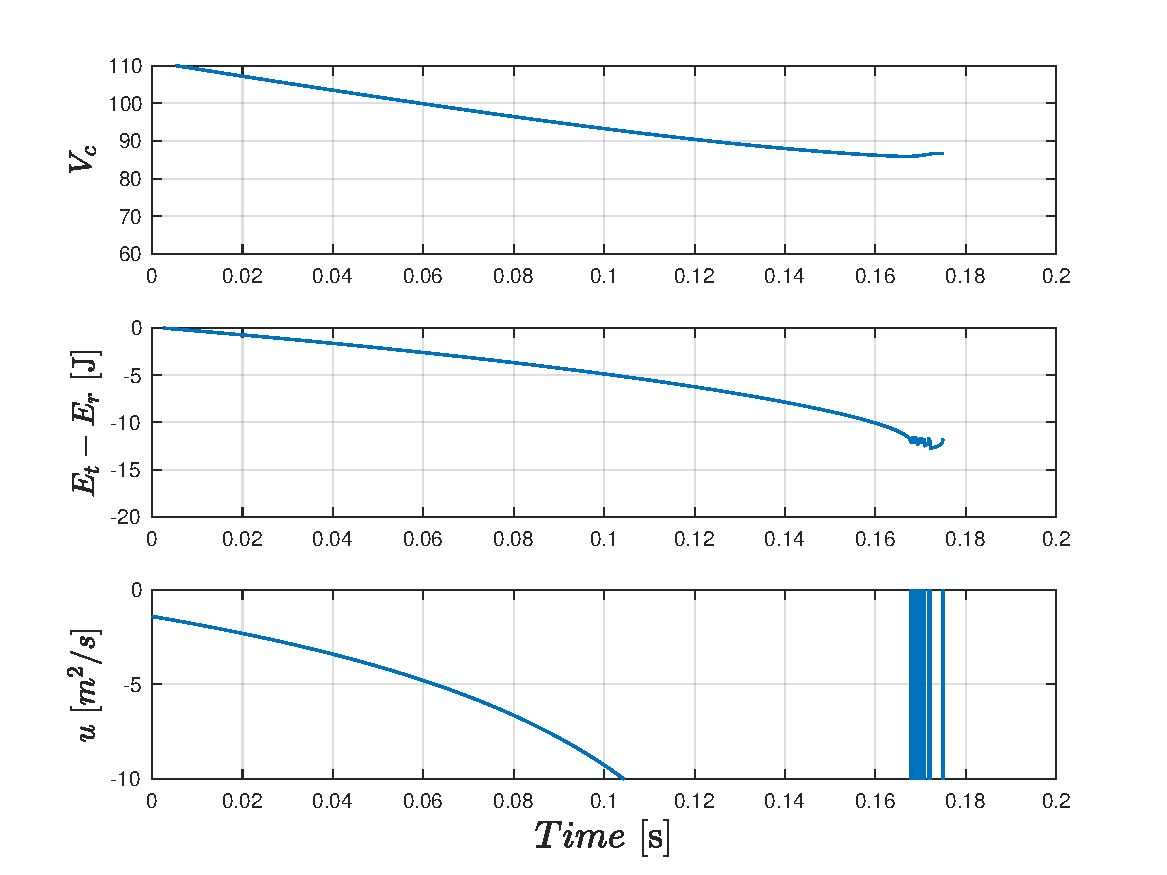
\includegraphics[width=1\linewidth]{figures/Total_Energy_Shaping/total_1.pdf}
 \caption{Time responses of $V_c$ , $E_T-E_r$, and $u$.}
\end{subfigure}
\caption{Controller \eqref{eq:tot-mech-energy-controller} encountered a singular point for initial state $\big(\theta(0),l(0),\dot{\theta}(0),\dot{l}(0)\big)$ $= (-\pi/6,2,0,4)$.}
\label{fig:singular_controller}
\end{figure}
\newpage
\subsection{Partial Energy Shaping}
For an initial state $\big(\theta(0),l(0),\dot{\theta}(0),\dot{l}(0)\big) = (-\pi/6,2,0,0)$, 
the numerical simulation results of the VLP under the controller \eqref{eq:controller-partial-energy-shaping} using the same control parameters defined above in \eqref{eq:control-parameters} are shown in Figs. \ref{fig:partial_1} and \ref{fig:partial_2}. Similarly, it is observed the convergence to zero for $V$ and $E_P-E_r$, and $V$ is non-increasing. As deducted from Fig. \ref{fig:partial_2}, the swing of the pendulum approaches the desired motion trajectory with $l$ converging to $l_r$.

In addition, it was validated numerically through Fig. \ref{fig:partial_3} that $V_{\delta}<V_{de}$ holds when $\delta$ satisfies \eqref{eq:delta-property} by presenting the plot $V_{\delta}-V_{de}$ with respect to $\delta$, giving that $\delta_m = 1.18$ from \eqref{eq:delta-property}. 

Another initial state was considered as $\big(\theta(0),l(0),\dot{\theta}(0),\dot{l}(0)\big) = (-\pi/3,l_{de},0,0)$ which satisfies $V_{\delta}<V_{de}$ with $V_{\delta} = 39.7$ and $V_{de} = 49.1$. The numerical simulation results of this initial condition are given in Figs. \ref{fig:partial_1b} and \ref{fig:partial_2b}. From them, it is observed that $V$, $E_P-E_r$ and $l-l_r$ converge to zero and that the closed-loop solution approaches the desired trajectory rather than the downward equilibrium point.
\begin{figure}[H]
    \centering
    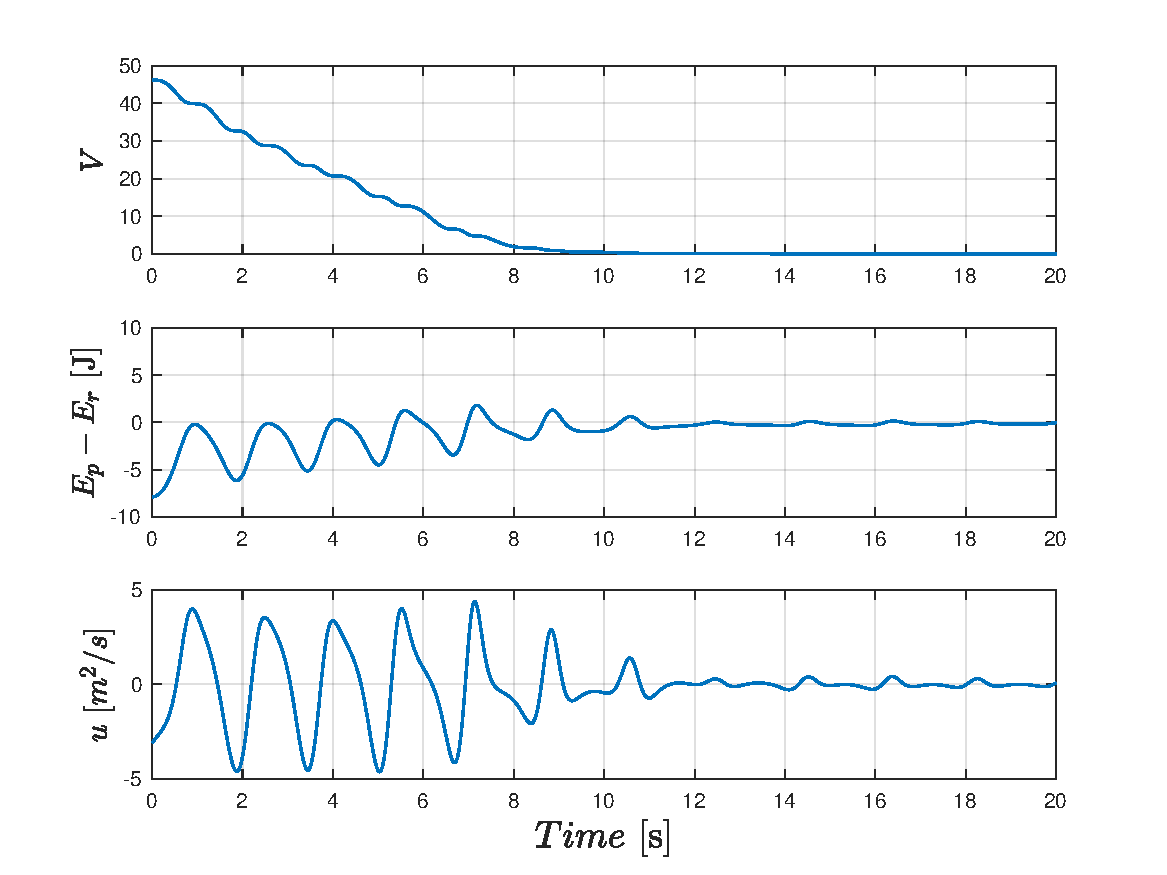
\includegraphics[scale = 0.6]{figures/Partial_Energy_Shaping/partial_1.pdf}
    \caption{Time responses of $V$, $E_P-E_r$ and $u$ with initial state  $\big(\theta(0), l(0), \dot{\theta}(0), \dot{l}(0)\big) = (-\pi/6, 2, 0, 0)$.}
    \label{fig:partial_1}
\end{figure}
\begin{figure}[H]
    \centering
    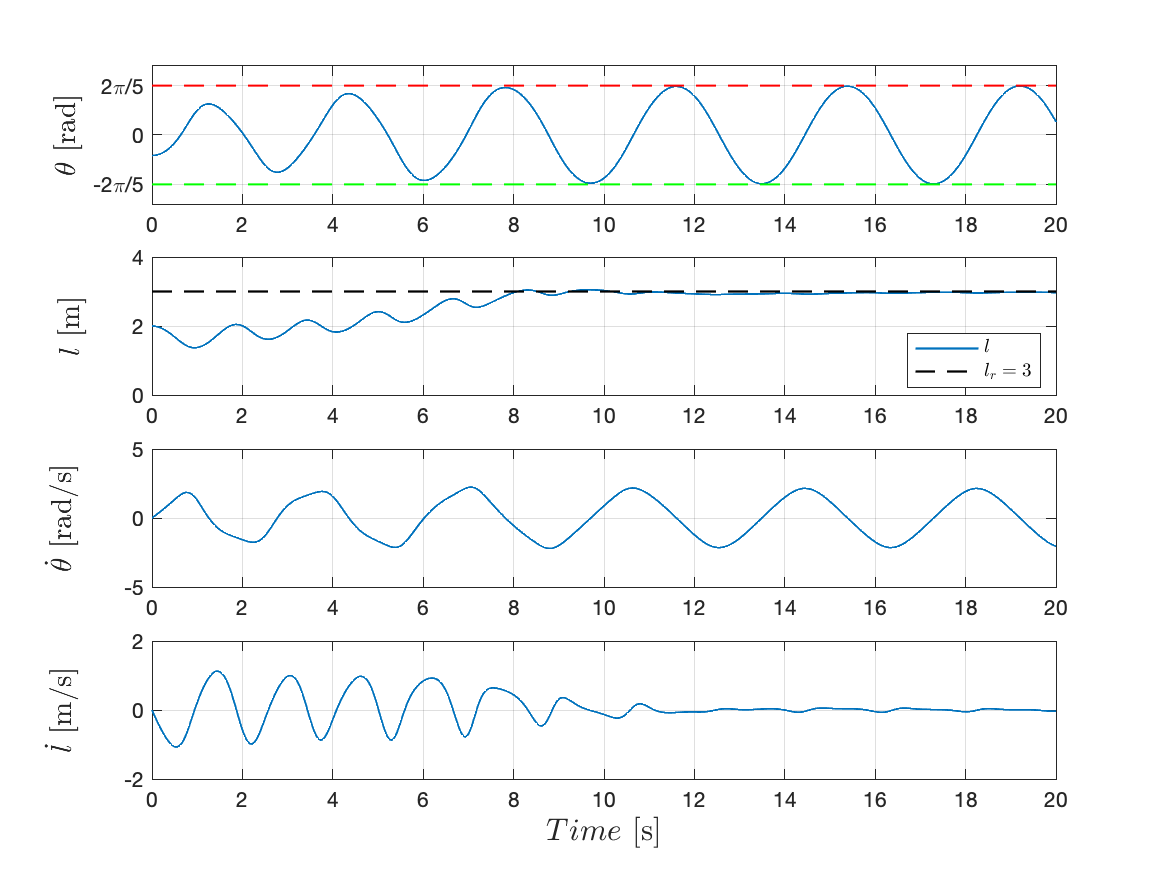
\includegraphics[scale = 0.6]{figures/Partial_Energy_Shaping/partial_2.pdf}
    \caption{Time responses of $\big(\theta,l,\dot{\theta},\dot{l}\big)$ with initial state $\big(\theta(0),l(0),\dot{\theta}(0),\dot{l}(0)\big) = (-\pi/6,2,0,0)$.}
    \label{fig:partial_2}
\end{figure}
\begin{figure}[H]
    \centering
    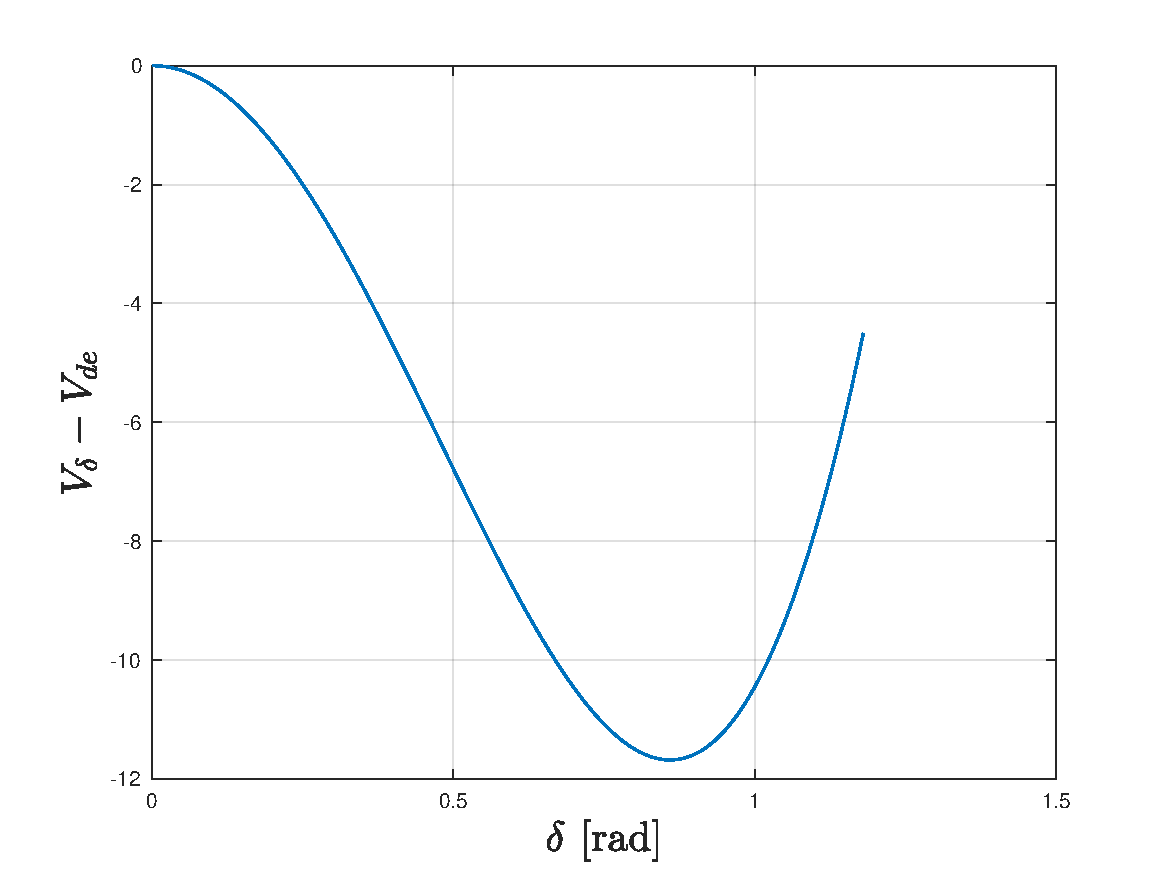
\includegraphics[scale = 0.6]{figures/Partial_Energy_Shaping/partial_3.pdf}
    \caption{$V_{\delta}-V_{de}$ with respect to $\delta$ in \eqref{eq:diff-lyapunov-V}.}
    \label{fig:partial_3}
\end{figure}
\begin{figure}[H]
    \centering
    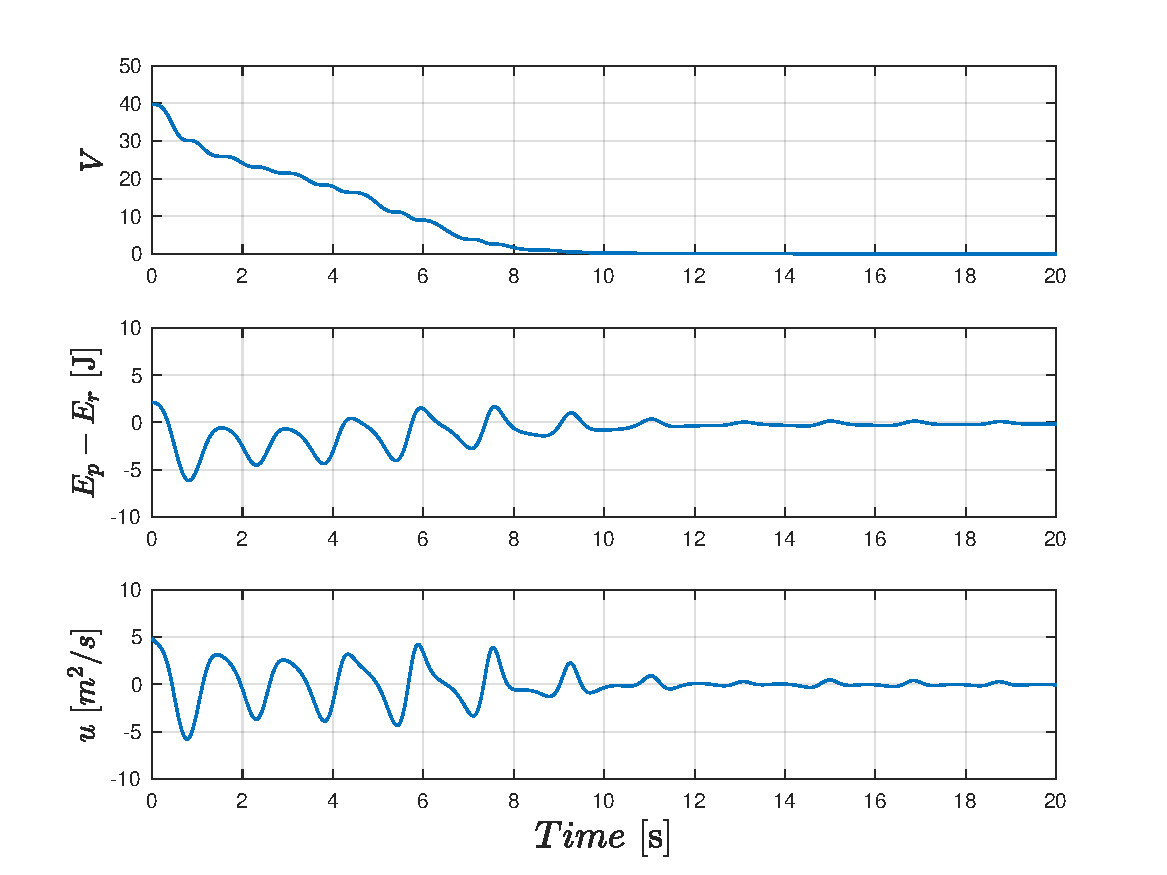
\includegraphics[scale = 0.6]{figures/Partial_Energy_Shaping/partial_1b.pdf}
    \caption{Time responses of $V$, $E_P-E_r$, and $u$ with initial state  $\big(\theta(0),l(0),\dot{\theta}(0),\dot{l}(0)\big) = (-\pi/3,l_{de},0,0)$}
    \label{fig:partial_1b}
\end{figure}
\begin{figure}[H]
    \centering
    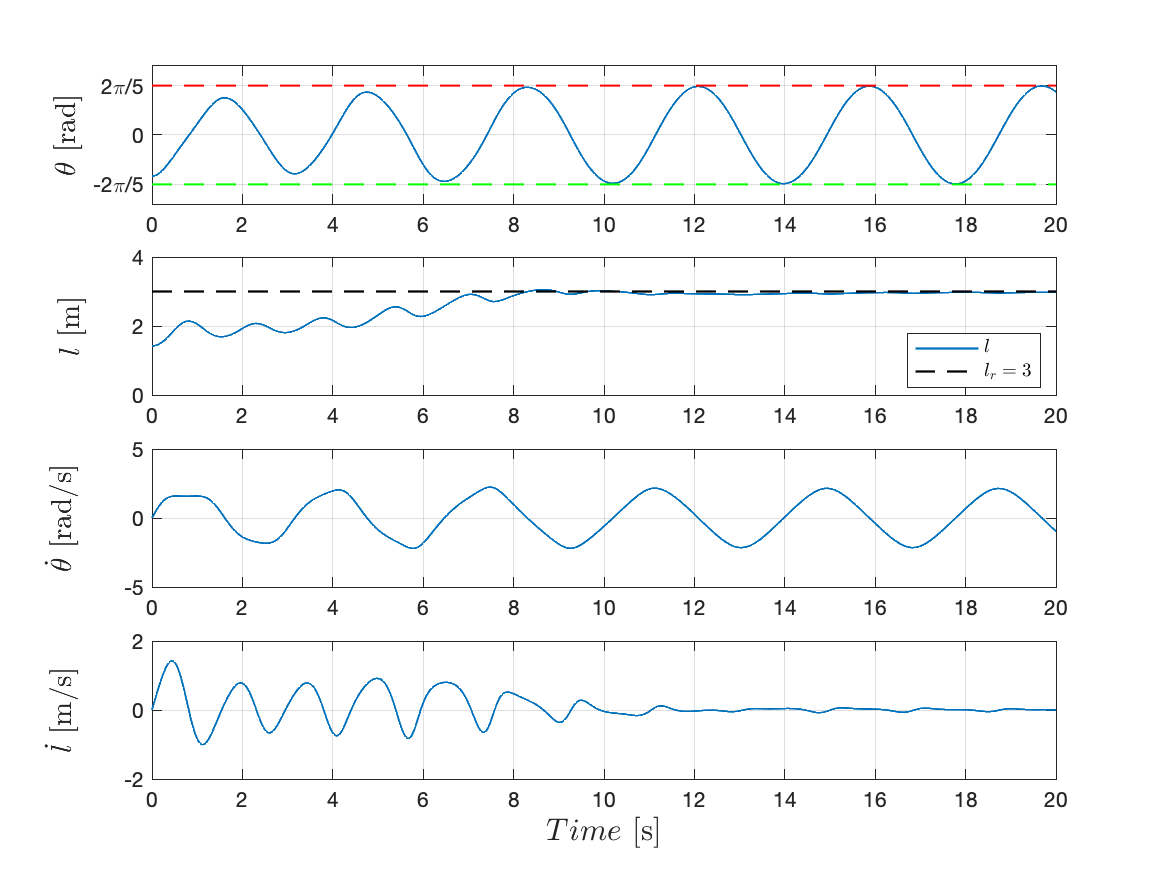
\includegraphics[scale = 0.6]{figures/Partial_Energy_Shaping/partial_2b.pdf}
    \caption{Time responses of $\big(\theta,l,\dot{\theta},\dot{l}\big)$ with initial state $(-\pi/3,l_{de},0,0)$.} 
    \label{fig:partial_2b}
\end{figure}

\end{document}